\begin{enumerate}
  \item Goal: management of network devices
  \item Pre-SDN approaches characterization: decentralized. List disadvantages (lack of: security, scalability, flexibility)
  \item Programmable approach to network devices management
  \item Logical separation of forwarding and routing packages
  \item Centralized approach to network devices management. Brief overview of 
  \item Standarized, open protocols to communicate with network devices
  \item Advantages of SDN
\end{enumerate}

\todo{How does TreeCaching interact with SDN?}

\vspace{1cm}
SEPARATOR
\vspace{1cm}

From TC paper INTRO:
\vspace{1cm}

\subsubsection{Abstract from TC}

We initiate the study of a natural and practically relevant new variant of
online caching where the to-be-cached items can have
dependencies.  We assume that the universe is a~tree~$T$ and items are tree
nodes; we require that if a node $v$ is cached then the whole subtree $T(v)$
rooted at $v$ is cached as well. This theoretical problem finds an immediate
application in the context of forwarding table optimization in IP routing and
software-defined networks.

We present an elegant online deterministic algorithm \ALG for this problem, and 
rigorously prove that its competitive ratio is 
$O(\textsc{height}(T) \cdot \kALG/(\kALG-\kOPT+1))$, where $\kALG$ and $\kOPT$
denote the cache sizes of an online and the optimal offline algorithm,
respectively. The result is optimal up to a factor of $O(\textsc{height}(T))$.



\subsubsection{Part of intro from TC}

One interesting application for our model arises in the context of modern IP
routers which need to store a rapidly increasing number of forwarding
rules~\cite{bgp-routeviews,steve-myth}. In \lref[Section]{sec:motivation}, we
give a glimpse of this application, discussing how tree caching algorithms can
be applied in existing systems to effectively reduce the memory requirements
on IP routers.

\subsubsection{Application (of TC): Minimizing Forwarding Tables in Routers}
\label{sec:motivation}

Dependencies among to-be-cached items arise in numerous settings and are a
natural refinement of many caching problems. To give a concrete example, one
important application for our tree-based dependency model arises in the context
of IP routers. In particular, the online tree caching problem we introduce in
this paper is motivated by router memory constraints in IP-based networks. The
material presented in this section serves for motivation, and is not necessary
for understanding the remainder of the paper.

Nowadays, routers have to store an~enormous number of forwarding rules: the
number of rules has doubled in the last six years~\cite{bgp-routeviews} and
the superlinear growth is likely to be sustained~\cite{steve-myth}. This
entails large costs for Internet Service Providers: fast router memory
(usually Ternary Content Addressable Memory (TCAM)) is expensive and
power-hungry~\cite{tcam-expensive}.  Many routers currently either operate at
(or beyond) the edge of their memory capacities. A~solution, which could delay
the need for expensive or impossible memory upgrades in routers, is to store
only a subset of rules in the actual router and store all rules on a~secondary
device (for example a commodity server with a large but slow
memory)~\cite{cacheflow,route-caching-flat,prefix-caching,fib-caching-non-overlapping,fibium-zipf}.

This solution is particularly attractive with the advent of Soft\-ware-Defined
Network (SDN) technology, which allows to manage the expensive memory using a
software controller~\cite{cacheflow,fibium-zipf}. In particular, our
theoretical model can describe real-world architectures
like~\cite{cacheflow,fibium-zipf},
that is, our model formalizes the underlying operational
problems of such architectures. Our 
algorithm, when applied in the context of such architectures, can 
hence be used to prolong the lifetime of IP routers.

\paragraph{Setup, positive requests, fetches and evictions.}

The setup (see~\cite{fibium-zipf} for a more technical discussion) depicted in
\lref[Figure]{fig:motivation} consists of two entities: the actual router 
(e.g., an OpenFlow switch) which caches only a~subset of all forwarding rules,
and the (SDN) controller, which keeps all rules in its less expensive and
slower memory. During runtime, packets arrive at the router, and if an
appropriate forwarding rule is found within the rules cached by the router,
then the packet is forwarded accordingly, and the associated cost is zero.
Otherwise, the packet has to be forwarded to the controller (where 
an~appropriate forwarding rule exists); this indirection costs~$1$. Hence, the
rules correspond to cacheable items and accesses to rules are modeled by
positive requests to the corresponding items. At some chosen points in time,
the caching algorithm run at the controller may decide to remove or add rules
to the cache. Any such change entails a~fixed cost $\alpha$.\footnote{This
cost corresponds to the transmission of a message from the controller to the
router as well as the update of internal data structures of the router. Such
an update of proprietary and vendor-dependent structures can be quite
costly~\cite{tcam-expensive-updates}, but the empirical studies show it to be
independent of the rule being updated~\cite{fib-updates}.}

\begin{figure}[t]
  \centering
  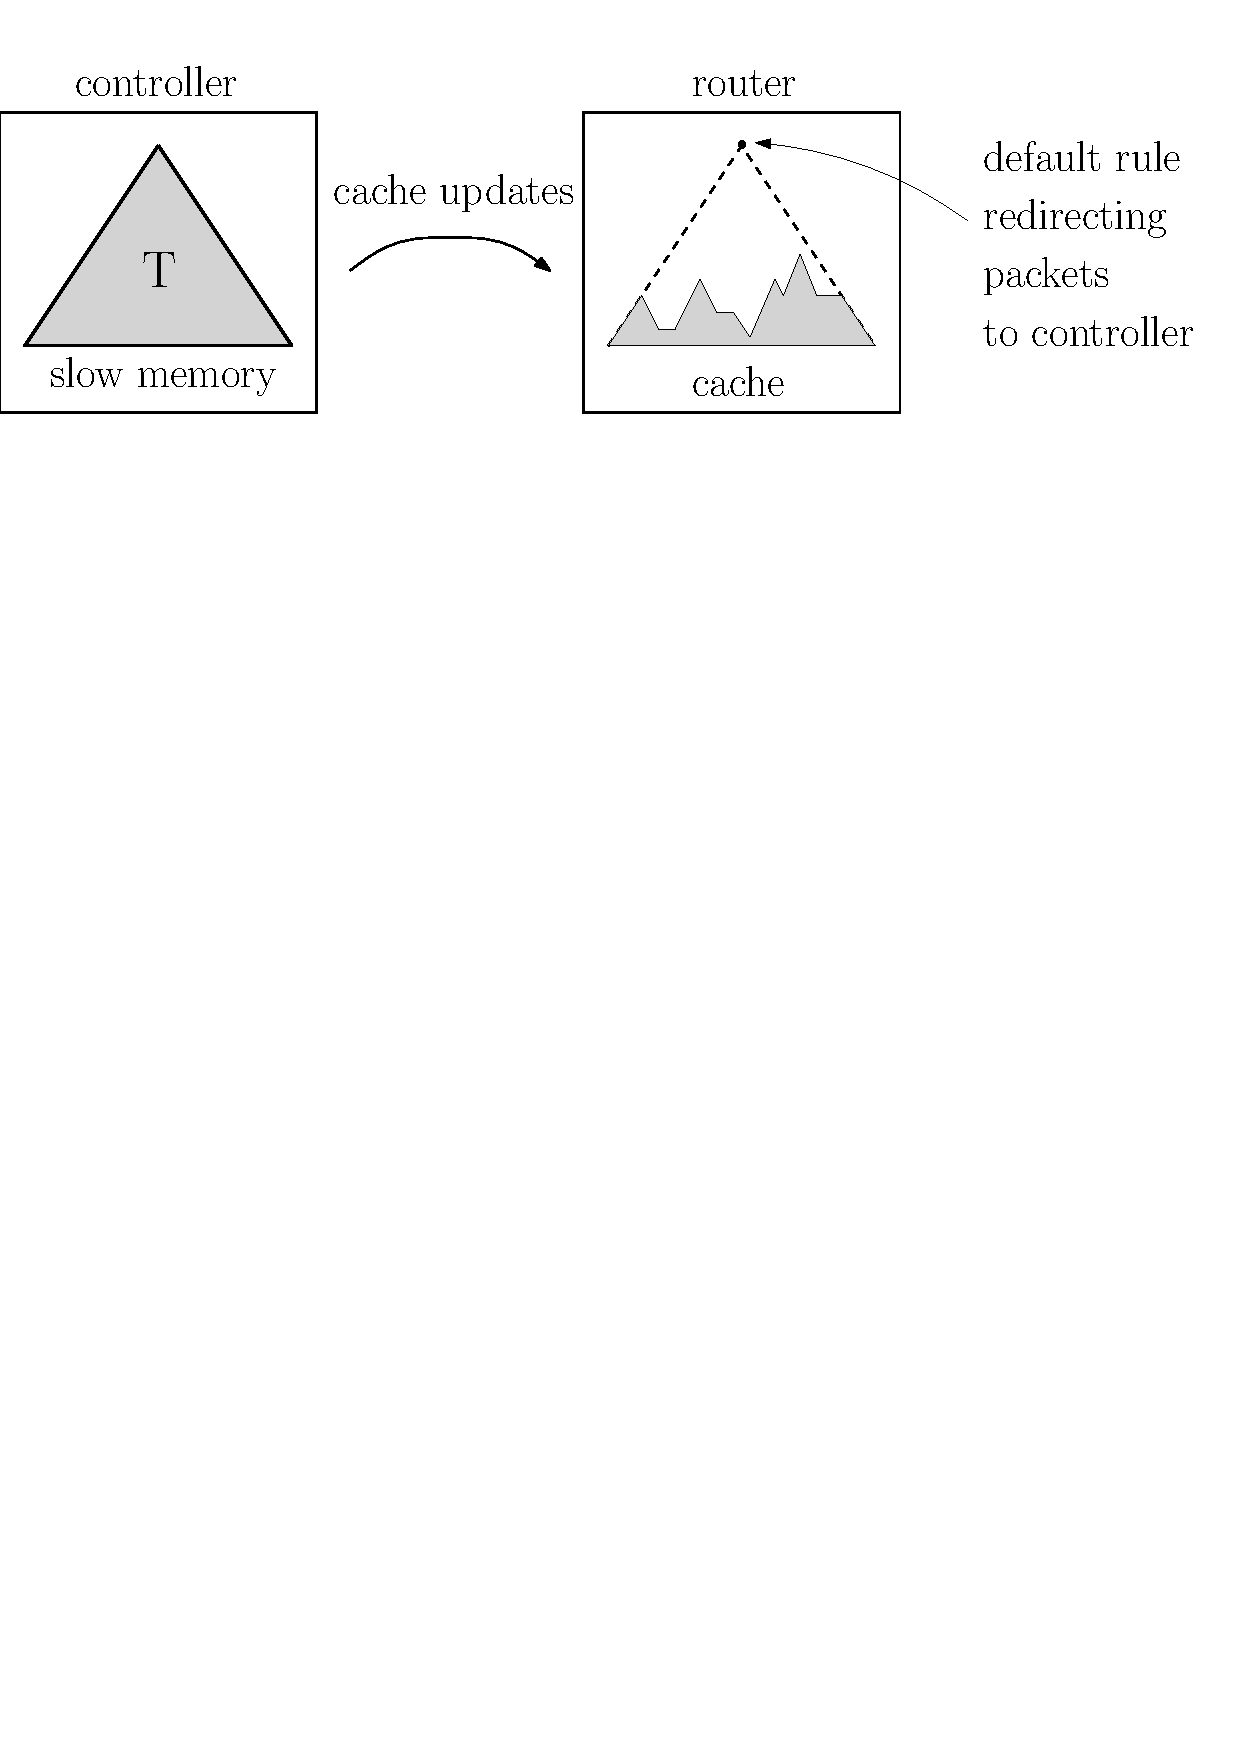
\includegraphics[width=0.9\columnwidth,keepaspectratio]{figs/cache-management/router}
  \caption{The router (\emph{right}) caches only a subset of all rules, and
  rules that are not cached are answered by the controller (\emph{left}) that
  keeps the whole tree of rules. Updates to the rules are passed by the
  controller to the router.}
  \label{fig:motivation}
\end{figure}


\paragraph{Tree dependencies.}

Note that the technical feasibility of this solution heavily depends on the
rule dependencies. In the most ubiquitous scenario, the rules are prefixes of
IP addresses (they are bit strings). Whenever a packet arrives, the router
follows a longest matching prefix (LMP) scheme: it searches for the rule that
is a~prefix of the destination IP of the packet and among matching rules it
chooses the longest one. In other words, if the prefixes corresponding to
rules are stored in the tree\footnote{We do not have to assume that they are
actually stored in a real tree; this tree is implicit in the LMP scheme.},
then the tree is traversed from the root downwards, and the last found rule is
used. This explains why we require the cached nodes to form a subforest:
leaving a less specific rule on the router while evicting a more specific one
(i.e., keeping a~tree node in cache while evicting its descendant) will result
in a~situation where packets will be forwarded according to the less specific
rule, and hence potentially exit through the wrong port. The LMP scheme also
ensures that the described approach is implementable: one could simply add
an~artificial rule at the tree root in the router (matching an empty prefix).
This ensures that when no actual matching rule is found in the router (in the
cache), the packet will be forwarded according to this artificial rule to the
controller that stores all the rules and can handle all packets appropriately.

So far, the papers on IP rule caching avoided dependencies either assuming
that rules do not overlap (a~tree has a single level)~\cite{route-caching-flat} 
or by preprocessing the tree, so that the rules become
non-overlapping~\cite{prefix-caching,fib-caching-non-overlapping}.
Unfortunately, this could lead to a large inflation of the routing table. A
notable exception is a recent solution called CacheFlow~\cite{cacheflow}. The
CacheFlow model supports dependencies even in the form of directed acyclic
graphs. However, CacheFlow was evaluated only experimentally, and no
worst-case guarantees were given on the overall cost of caching. Our work
provides theoretical foundations for respecting tree dependencies.

\paragraph{Negative requests.}

Additionally, a rule may need to be updated. For example, due to a~change
communicated by a dynamic routing protocol (e.g., BGP) the action defined by
a~rule has to be modified. In either case, we have to update the rules at the
controller: we assume that this cost is zero. (This cost is unavoidable for
any algorithm, so such an assumption makes our problem only more difficult.)
Furthermore, if the rule is also stored at the router, then we have to pay a~fixed
cost of $\alpha$ for updating the router (see the remark for the cost of
fetches and evictions). Such penalties can be easily simulated in our model:
we issue a~sequence of $\alpha$ negative requests to the updated node.  It is
straightforward to show that the costs in these two models can differ by a
factor of at most $2$. For a~formal argument, see
\lref[Appendix]{sec:bisimulation}.

\paragraph{Implementability.}

Note that the whole input (fed to a tree caching algorithm) is created at the
controller: positive requests are caused by cache misses (which redirect
packet to the controller) and batches of $\alpha$ negative requests are caused
by updates sent to the dynamic routing algorithm run at the controller.
Therefore, the whole tree caching algorithm can be implemented in software
in the controller only. Furthermore, our algorithm is a simple counter-based
scheme, which can be implemented efficiently and also fine-tuned for speed,
see \lref[Section]{sec:implementing_counters}.

\paragraph{Other work on forwarding table minimization.}

Other approaches for minimizing the number of stored rules were mostly based
on \emph{rules compression (aggregation)}, where the set of rules was replaced
by another equivalent and smaller set. Optimal aggregation of a fixed routing
table can be achieved by dynamic
programming~\cite{ortc,fib-compression-two-dimensional}, but the main
challenge lies in balancing the achieved compression and the amount of changes
to the routing table in the presence of \emph{updates} to this table. While
many practical heuristics have been devised by the networking community for
this problem~\cite{mms,fib-compression-fifa,fib-compression-globecom10,fib-compression-infocom13,fib-sigcomm,fib-compression-smalta,fib-compression-infocom10},
worst-case analyses were presented only for some restricted
scenarios~\cite{fib-icdcs,fib-sirocco}. Combining rules compression and rules
caching is so far an unexplored area.

